\documentclass[a4paper]{report}

\setcounter{tocdepth}{4}
\setcounter{secnumdepth}{3}
\newcommand\figref{Figure~\ref}

\usepackage{longtable}
\usepackage{comment}
\usepackage{multirow}
\usepackage[utf8]{inputenc}
\usepackage[T1]{fontenc}
\usepackage[pdftex]{graphicx}
\usepackage{xcolor}
%\usepackage[capposition=top]{floatrow}   
% \usepackage[margin=1in]{geometry} 
\usepackage{subfigure}

\usepackage[english]{babel} 


\usepackage{amsmath}
\usepackage{amssymb}
\usepackage{amsthm}
\DeclareMathOperator{\Tr}{Tr}
\usepackage{bigints}

%\usepackage{subcaption}

\usepackage{titlesec}
\newcommand{\sectionbreak}{\clearpage}
\usepackage{lmodern}
\graphicspath{{../img/}}
 \DeclareGraphicsExtensions{.pdf,.jpg,.png}
\usepackage{microtype}


\usepackage[hidelinks,plainpages=false,pageanchor=false]{hyperref}
%\hypersetup{pageanchor=false}
\begin{document}


\begin{titlepage}
\begin{center}

% Upper part of the page. The '~' is needed because \\
% only works if a paragraph has started.


\textsc{\LARGE Singularity Graph Build}\\[1.5cm]

\textsc{\Large Report}\\[0.5cm]

% Title

{ \huge \bfseries TODO list \\[0.4cm] }



% Author and supervisor
\begin{minipage}{0.4\textwidth}
\begin{flushleft} \large
%\emph{Ph.D.:}\\
Ana-Maria \textsc{Vintescu}
\end{flushleft}
\end{minipage}
\begin{minipage}{0.4\textwidth}
\begin{flushright} \large
Franck \textsc{Ledoux}
\end{flushright}
\end{minipage}


% Bottom of the page
\date{} % blank date

\end{center}
\end{titlepage}


\date{} % blank date



\renewcommand{\thesection}{\arabic{section}}


\tableofcontents{}

\setcounter{tocdepth}{4}
\newpage
\section{Introduction}

{This document presents known bugs, TODO lists and possible improvements of the code for the Singularity Graph Extraction.
}



\bigskip


\section{TODO list}
{ 

\begin{itemize}
\item For all streamline computation methods (\textcolor{blue}{$SingularityGraphBuilder2D::growLine()$} , \textcolor{blue}{$SingularityGraphBuilder2D::computeStreamLine()$}), it is currently tested if we reach on the confusing ball of a different singularity ((\textcolor{green}{$m\_faces\_to\_singularity\_on\_surf$})) or if we reach the boundary.
If \textcolor{green}{$m\_build\_geometric\_singularities==true$}, it should be tested also if we reach in one of those faces (\textcolor{green}{$singOrGeomFaces$}) and if so, to connect.
\newline
\item \textcolor{blue}{$SingularityGraphBuilder2D::computeSingPointInfo()$} 
The singularity point is always placed at the center of the triangle; it should be placed at the right position.
\newline
\item \textcolor{blue}{$SingularityGraphBuilder2D::$} \textcolor{blue}{$createSingularityLinesSimultaneousStart()$} and \textcolor{blue}{$SingularityGraphBuilder2D::$} \textcolor{blue}{$ createSingularityLinesSimultaneousStartRK4()$}
Although improbable, it could happen that a streamline arrives in the confusing ball of a different singularity (and they haven't been within the \textcolor{green}{$thresholdStreamLineDist$} already, so they weren't considered to connect). In this case we should proceed exactly as in the original algorithm: connect the slots and add the singularity line to the graph.
\newline
\item \textcolor{blue}{$SingularityGraphBuilder2D::createSingularityLinesShortestPaths()$} 
For each slot we will try to detect the "shortest path" towards all other slots except the slots belonging to the same singularity; As well, in the optimization procedure, the variables corresponding to the streamlines between slots of the same singularity will be set to $0$. However, in certain cases this shouldn't be valid (ex: close-to-circular mesh with a hole inside where a single singularity point is detected and where the frame field is also circular; in this case we would expect that one of the streamlines should connect two slots of the same singularity).
\item  Before \textcolor{blue}{$SingularityGraphBuilder2D::getShortestPathBtwFacesOptimized$}, 
if we have already detected streamlines, we must also mark them for the \textcolor{green}{$IllegalCross$} check (walk along the \textcolor{green}{$line_triangles$} and add them to \textcolor{green}{$isTraversedFaceCompVector$}).
\item \textcolor{blue}{$SingularityGraphBuilder2D::createSingularityLinesShortestPaths()$} 
\newline
At the beginning of the algorithm, when we advance with RK4 until we reach different faces; if we reach boundary, we must check if the boundary intersection point is very close to a geometric singularity and if the streamline is aligned with one of the geometric singularity's slots. If so, that won't be a boundary singularity line, but a singularity line between two slots of two singularities.
\item Inside \textcolor{blue}{$SingularityGraphBuilder2D::getShortestPathBtwFacesOptimized()$}, when we check whether the conditions are met to connect to the boundary (the last segment of the streamline and the boundary normal (at that end point) should be near collinear). However, if the end point is inside the confusing ball of a geometric singularity we discard the boundary streamline. But we should discard it only if a) the streamline end point and the geometric singularity are very close and also if b) the last segment of the streamline and one of the geometric singularity's slots are aligned (\textcolor{green}{$if(singOrGeomFaces[paths2[tk]])\ \ toConsider = false;$} ).
\item
\end{itemize}
\begin{comment}

\begin{equation}
J_f=U \Sigma V^T = U  \begin{pmatrix}
\sigma_1 & 0  \\
0 & \sigma_2 \\
0 & 0
\end{pmatrix} V^T
\end{equation}
\end{comment}

}


\newpage
\section{Known bugs}
{%( \textcolor{green}{createSingularityLinesShortestPaths()})

%\begin{equation}
% \underbrace{\bigintsss _{S} det(\textbf{J}) ds}_\text{area of the surface}  = \underbrace{\frac{1}{2} \bigintsss _{S} ||f_u||^2+ ||f_v^2||  ds}_\text{Dirichle's energy} - \underbrace{\frac{1}{2} \bigintsss _{S} ||f_v-rot_{90}(f_u X)||^2}_\text{conformal energy}
%\end{equation}

\begin{itemize}
	\item[1.] \textcolor{blue}{$SingularityGraphBuilder2D::initConfusingBalls$}
	\newline
	Since this function is applied iteratively to all singular points, if two such points are 		very close to one another and/or the distance radius 
	(\textcolor{green}{$m_confusing_distance$}) has a high value, 
	the latest detected confusing ball could 
	override a 	previous one.
	%%%%%%%%%%%%%%%%%%%%%%%%%%%%%%%%%%%%%%%%%%%%%%%%%%%%%%%%%%%%%%%%%%%%%%%%%%%%%%%%%%%%%%%%
	\item[2.] 
	\textcolor{blue}{$SingularityGraphBuilder2D::createSingularityLinesShortestPaths$}
	\newline
	At the beginning (iteratively, for all singularities) we depart from a singularity along 			its slots' directions until we reach different faces. The main purpose here is to have 
	the end points of all streamlines departing from the same singularity inside different 			triangles (they depart from the same triangle - the singular triangle). 
	At each such iteration, if we land on the boundary or if we arrive onto the confusing 
	ball of a different singularity (and all conditions are met), we create the singularity 			line and freeze the slot. However, 
	\begin{itemize}
	%%%%%%%%%%%%%%%%%%%%%%%%%%%%%%%%%%%%%%%%%%%%%%%%%%%%%%%%%%%%%%%%%%%%%%%%%%%%%%%%%%%%%%%%
		\item[a)] if two such streamlines meet the conditions for connecting (the distance between them is smaller than \textcolor{green}{$thresholdStreamLineDist$}, as in \textcolor{blue}{$SingularityGraphBuilder2D::createSingularityLinesSimultaneousStartRK4$}), we do not connect them. $\rightarrow$ this should be corrected.
%%%%%%%%%%%%%%%%%%%%%%%%%%%%%%%%%%%%%%%%%%%%%%%%%%%%%%%%%%%%%%%%%%%%%%%%%%%%%%%%%%%%%%%%
		\item[b)] Even if we would apply the strategy above, we might still have a problem: here we treat iteratively each singularity. Therefore, in certain conditions (2 singularities that are too close to one another, coarse mesh, high RK4 propagation step), we could simply "miss" the connection. This happens because one streamline could be advanced too much (passing its possible proximity with another streamline), since they are advanced iteratively. See Fig.~\ref{fig:ex1}.
\begin{figure}[!h]
            \centering
            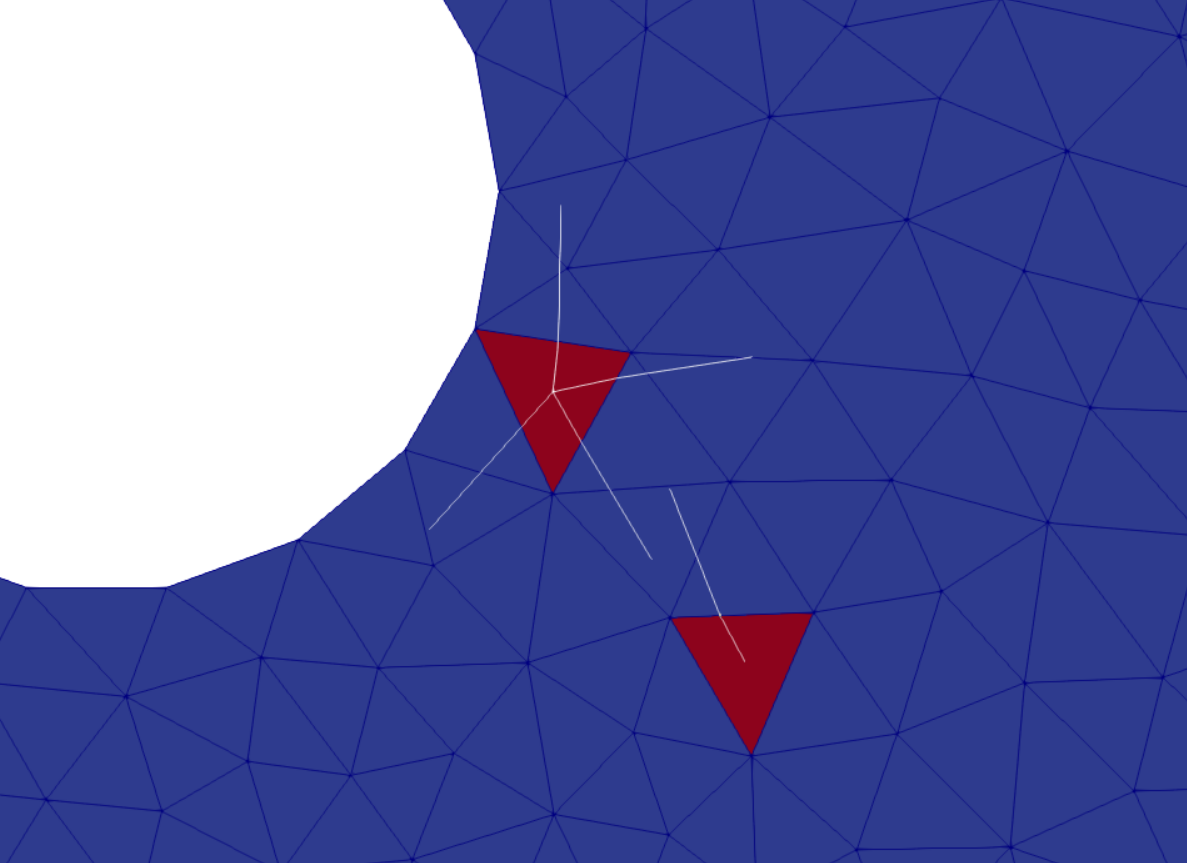
\includegraphics[width=0.5\textwidth]{ex1}
            \caption{\small problem 2b)}  
            \label{fig:ex1}
        \end{figure}
	\end{itemize}
	%%%%%%%%%%%%%%%%%%%%%%%%%%%%%%%%%%%%%%%%%%%%%%%%%%%%%%%%%%%%%%%%%%%%%%%%%%%%%%%%%%%%%%%%
	\item[3.] \textcolor{blue}{$SingularityGraph::buildCurveSurfacePatchs()$} In some cases, wrong results.
	Example: mesh HolesInSquare2, \textcolor{green}{$AStrategy == shortestPaths$}; In 				Fig.~\ref{fig:ex2} the entire area with red lines is considered as a single patch.
	\begin{figure}[!ht]
    	\centering
        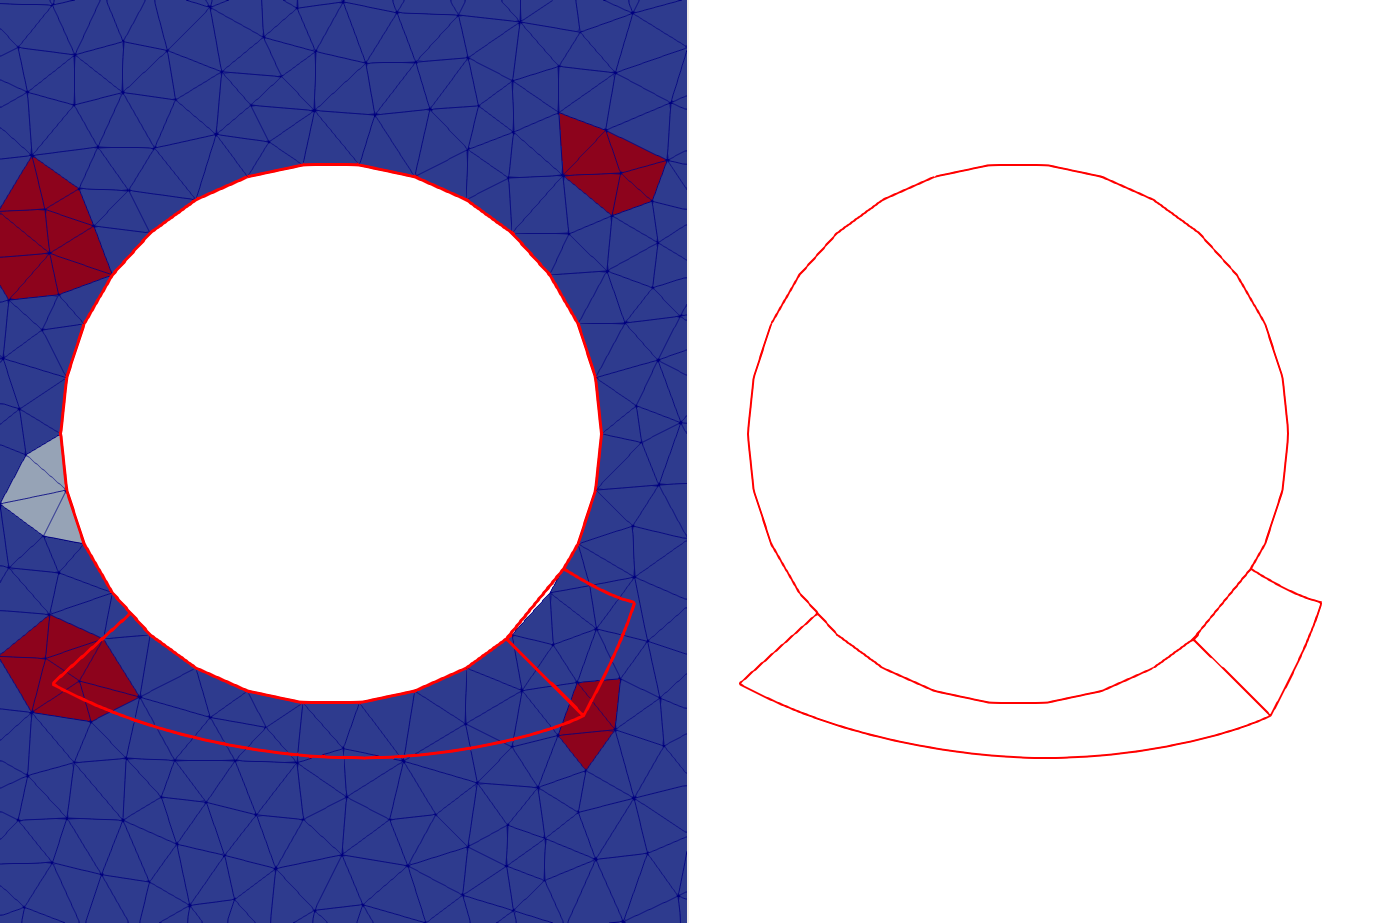
\includegraphics[width=0.5\textwidth]{ex2}
        \caption{\small problem 3)}  
        \label{fig:ex2}	
    \end{figure}
    
%%%%%%%%%%%%%%%%%%%%%%%%%%%%%%%%%%%%%%%%%%%%%%%%%%%%%%%%%%%%%%%%%%%%%%%%%%%%%%%%%%%%%%%%        
	\item[4.] \textcolor{blue}{$SingularityGraphBuilder2D::getShortestPathBtwFacesOptimized()$}
	 Since from propagating from triangle to triangle we use \textcolor{green}{$Cross2D::closestComponentVector()$}, it can be problematic if the closest component vector makes a $45^{\circ}$ angle with the vector.
\end{itemize}
\begin{comment}

\begin{figure}[H]

\includegraphics[width=0.5\textwidth]{img/mesh_completion.png}
\caption{Mesh Completion \cite{KraevoyS05}}
\floatfoot{Completing a head: (a,d) the input mesh, (b,e) the template, (d,f) the completed model}
\end{figure}

\begin{figure}[H]
\includegraphics[width=0.9\textwidth]{img/remesh-cpcr.png}
\caption{Remeshing \cite{Kraevoy2004}}
\floatfoot{a) source mesh, b) target mesh after initial projection, c) smoothing step, d) final mesh}
\end{figure}
\end{comment}
}






 \newpage
\section{Possible Improvements}
{
\begin{itemize}
\item[•] \textcolor{blue}{$SingularityLine::healOrientation()$}
\newline
Now this is performed geometrically; this should be performed topologically, otherwise it is prone to errors. If the mesh is consistently oriented (in a preprocessing step). this topological procedure is straightforward.
\item[•] \textcolor{blue}{$SingularityGraphBuilder2D::computeFace2FaceInfo()$}
\newline
Assumes the mesh is a manifold.
\newline
\textcolor{green}{$face2Face_neighbours_by_verts$} and \textcolor{green}{$newNode2NewNodeNeighbours$} can be detected in a cheaper manner.
\newline
\textcolor{green}{$face2FaceDeviation$} - finish computing(will be used in $3D$).
\newline
\item[•] \textcolor{blue}{$SingularityGraphBuilder2D$}
\newline
A value is computed (\textcolor{green}{$temp\_epsilon$} $ = 3\% \ mean\_edge\_length$). this is further used in several functions (detect if point is in triangle, detect if two segments intersect, etc. ). This has been chosen over the globally defined \textcolor{green}{$math::Constants::EPSILON$}.
\end{itemize}


}


 \newpage
\section{Comments}
{
\begin{itemize}
\item[•] In $gmds: Tests\_pvsm$ file \textcolor{red}{$HIS-testOpt$} contains the list of tested examples and for some of them it is indicated if our algorithm (ShortestPaths) works and if not , the reason why it isn't working. 
\item[•] In \textcolor{red}{$SingularityGraphBuilder2D.h$} the boolean variable \textcolor{green}{$visualizeShortestPaths$} can be found. If this is set to true the algorithm will write a vtk file $"ShortestPaths_a-b.vtk"$ for each pair of slots $a$ and $b$. 
In the case of very large meshes or with many singularities this can be a problem $\rightarrow$  set \textcolor{green}{$visualizeShortestPaths = false$}.
\item[•] \textcolor{blue}{$SingularityGraphBuilder2D::redefineOneConfusingBall()$} and \textcolor{blue}{$SingularityGraphBuilder2D::initConfusingBalls()$}
\newline
If the distance between two singularity points is smaller than the defined radius for the confusing ball, some faces will be considered as being in the confusing ball of only one of the   two singularities.
\item[•]
\end{itemize}
}

\bibliographystyle{plain}
%\bibliography{library.bib}

\bibliography{./library}

%\addbibresource{library.bib}


\end{document}









